% !TeX encoding = UTF-8
% !TEX root = ./presentation.tex

   \begin{frame}{\Wearable: Capacete para Segurança de Ciclistas}{Leitura de Sensores}
      \scalebox{.7}{
         \begin{algorithm}[H]
             \SetKwData{data}{datas}
             \SetKwData{typew}{type\_warning}
             \SetKwData{sx}{sensor$_i$}
             \SetKwFunction{leSensores}{read\_sensors}
             \SetKwFunction{preprocess}{pre\_process}
             \SetKwFunction{process}{process}
             \SetKwFunction{atuacao}{operate}
             \SetKwFunction{finterrupt}{do\_interruption}
             \SetKwFunction{bu}{backup}
             \SetKwFunction{leds}{do\_leds\_warning}
             \SetKwData{btypew}{buffer\_type\_warning}
             
             \BlankLine
             \KwIn{sensors reads.}
             \KwOut{backups and interruptions signals.}
             \BlankLine
             
             \Begin{
                 \tcp{statements}
                 \sx\tcp*{$i$ information's source}
                 \data\tcp*{data's matrix before handling}
                 \typew\tcp*{type of warning to do to user}
                 \BlankLine
                 
                 \While{wearable mode on}{
                     \data $\leftarrow$ \leSensores{\sx}\;
                     \BlankLine
                     
                     \tcp{process the datas}
                     \typew $\leftarrow$ \process{\data}\;
                     
                     \BlankLine
                     \If{\typew $=$ dangerous}{
                         \finterrupt{\typew}\;
                         \leds{\btypew}\;
                     }                  
                     
                     \BlankLine
                     \bu{\data}\;
                 }
                 \BlankLine
             }
             
             \caption{Wearable 2 - Procedimento que realiza leituras de sensores e armazena seus dados em memória não-volátil.}
             \label{alg:wearable2_leituras}
         \end{algorithm}
      }
\end{frame}

   
   \begin{frame}{Procedimento Analítico Proposto}
      \scalebox{.78}{  
         \begin{algorithm}[H]
            \SetKwData{itt}{it}
            \SetKwData{pl}{partition\_list}
            \SetKwData{complexSet}{how\_complex\_set\_is}
            \SetKwData{md}{matriz\_dados}
            \SetKwData{complexSet}{how\_complex\_set\_is}
            \SetKwFunction{graph}{make\_graph}
            \SetKwFunction{porte}{analyse\_complex\_set}
            \SetKwFunction{synth}{synthesize}
            \SetKwFunction{resources}{resource\_used}
            \SetKwFunction{die}{die\_used}
            \SetKwFunction{energy}{energy\_spent}
            \SetKwFunction{profiling}{profile}
            \SetKwFunction{performance}{performance\_analysis}
            \SetKwFunction{factor}{complexity\_factor}
            \SetKwFunction{ilp}{integer\_linear\_solve}
            \SetKwFunction{heuristic}{heuristic}
            
            %\BlankLine
            \Begin{
               
               \BlankLine
               \profiling{}\;
               \BlankLine
               
               \tcp{extration project analyses}
               \graph{Flow Control Graph}\;
               \graph{Call Graph}\;
               %\complexSet $\leftarrow$ \porte{}\tcp*{verify if it is a big project}
               
               \BlankLine
               
               \If{exist partitions that can be synthesized}{
                  \ForEach{partition project:\itt $\in$ \pl}{
                     \synth{\itt}\;
                     \BlankLine
                     \resources{\itt}\tcp*{analysis after synth}
                     \die{\itt}\;
                     \energy{\itt}\;
                     %\BlankLine
                     
                     
                     \performance{\itt}\;
                  }
                  \BlankLine
                  
                  %\uIf(\tcp*[f]{verify if it is a small project}){\factor{\complexSet}}{
                  \ilp{\pl}\tcp*{analyse quantitatively each $ \Gamma $}
                  %}
                  %\lElse{
                  %\heuristic{\pl}\;
                  %}
               }
            }
            \caption{Metodologia para avaliação de wearables.}
         \end{algorithm}
      }
   \end{frame}

   \begin{frame}{\Wearable: Capacete para Segurança de Ciclistas}
        \vspace{-0.8em}
      
      \begin{figure}[h] \centering
         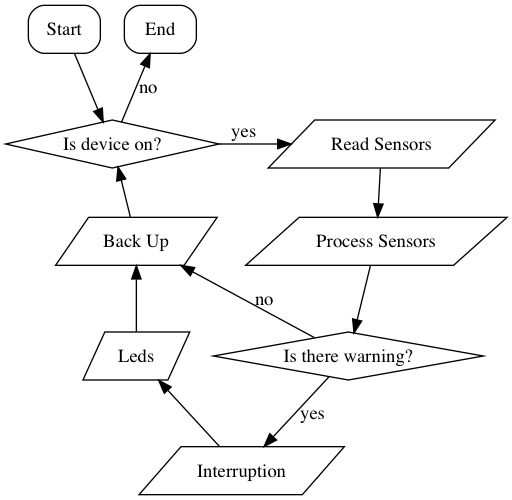
\includegraphics[width=0.67\textwidth]{img/capacete.png}
         \vspace{-1em}
         \caption{Grafo do projeto Wearable.}
      \end{figure}
      
   \end{frame}

    \begin{frame}{\Wearable: Capacete para Segurança de Ciclistas}
    \vspace{-0.8em}
    
        \begin{figure}[h] \centering
        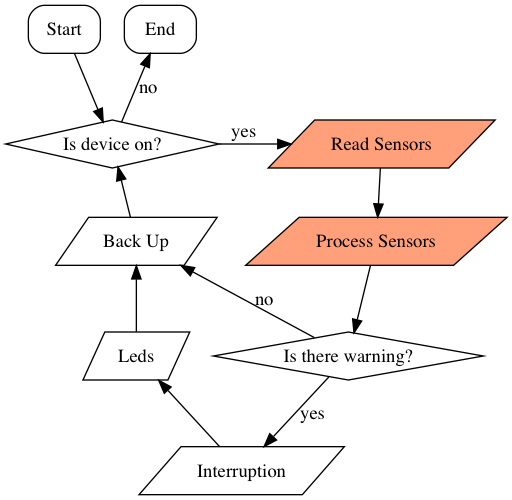
\includegraphics[width=0.67\textwidth]{img/capacete2.png}
        \vspace{-1em}
        \caption{Grafo do projeto Wearable.}
        \end{figure}
    \end{frame}


    \begin{frame}{\Wearable: Capacete para Segurança de Ciclistas}
        \vspace{-0.8em}
        
        \begin{columns}
            \begin{column}{0.6\textwidth}
                
                \begin{figure}[h] \centering
                    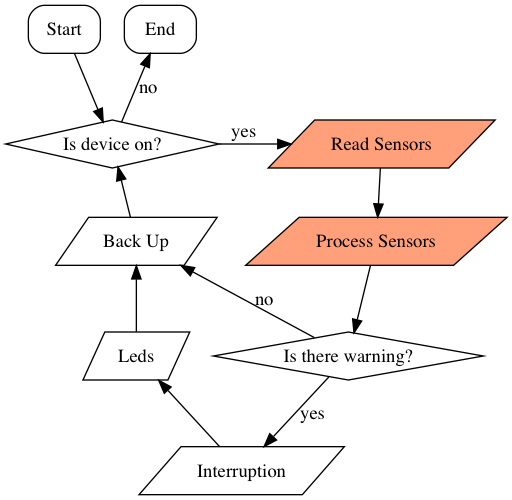
\includegraphics[width=1\textwidth]{img/capacete2.png}
                    \vspace{-1em}
                    \caption{Grafo do projeto Wearable.}
                \end{figure}
            \end{column}
            \begin{column}{0.4\textwidth}
                \vspace{-1cm}
                \begin{itemize}
                    \setlength{\itemsep}{1.4em}
                    \item Análise de $1..3$ sensores
                    \begin{enumerate}
                        \setlength{\itemsep}{0.8em}
                        \item Ao utilizar vários sensores, tem-se um \textbf{espaço}.
                    \end{enumerate}
                    \item Funções com complexidade diferentes
                    \begin{itemize}
                        \item Testar a aplicação utilizando $\mathcal{O}(1)$, $\mathcal{O}(n\log n)$ e $\mathcal{O}(n^2)$.
                    \end{itemize}
                \end{itemize}
                
            \end{column}
        \end{columns}
    \end{frame}
